\documentclass[10pt]{beamer}

\usetheme{CambridgeUS}
\usepackage[english, russian]{babel}
\usepackage[utf8]{inputenc}
\usepackage{caption}
\usepackage{etoolbox}
\usepackage{multicol}
\usepackage{listings}
\usepackage{color}

\definecolor{mygreen}{rgb}{0,0.6,0}
\lstset{
  basicstyle=\ttfamily\footnotesize,        % the size of the fonts that are used for the code
  breaklines=true,                 % automatic line breaking only at whitespace
  captionpos=b,                    % sets the caption-position to bottom
  commentstyle=\color{mygreen},    % comment style
  keywordstyle=\color{blue},       % keyword style
  stringstyle=\color{red},     % string literal style
  showstringspaces=false,
  morekeywords={include, printf},
  texcl=true     %<---- added
}

\title[Ввдение в обработку естественных языков]{Языковые модели}
\author[Гусев Илья]{Гусев Илья}
\institute[МФТИ] 
{Московский физико-технический институт\\*}
\date{Москва, 2018}
\subject{Computer Science}

\begin{document}

\begin{frame}
  \titlepage
\end{frame}

\begin{frame}{Содержание}
\tableofcontents
\end{frame}

\section{Языковые модели}

\begin{frame}{Языковые модели}
Статистичская языковая модель (statistical language model) - вероятностное распределение над последовательностями слов $P(w_1, ..., w_m)$.\\
Применения:
\begin{enumerate}
    \item Распознвание речи (ASR)
    \item Машинный перевод (MT)
    \item PoS-tagging
    \item OCR
    \item Распознавание рукописных текстов
    \item Классификация текстов
\end{enumerate}
В целом, нужны везде, где речь идёт о последовательностях слов. Мы рассматриваем языковые модели именно на уровне слов, но бывают ещё и char-level и subword модели.
\end{frame}

\begin{frame}{Train, validation(dev), test}
\begin{itemize}
    \item Для обучения практически любой языковой модели нужен большой корпус. Достаточно иметь тексты, разбитые на токены. \\
    \item Train выборка - собираем статистику или учим модель.\\
    \item Validation(dev) выборка - выбираем гиперпараметры модели, таким образом, чтобы языковая модель лучше работала на этой выборке.\\
    \item Test выборка - оцениваем качество языковой модели. \\
\end{itemize}
\end{frame}

\begin{frame}{Перплексия}
$$ PP(W) = P(w_1w_2...w_N)^{-\frac{1}{N}} = \sqrt[N]{\frac{1}{P(w_1w_2...w_N)}} $$
Средневзвешенное количество слов, которые могут следовать за данным словом.

Пример: язык из 9 символов $0, 2, ..., 9$, для каждого из них $P = \frac{1}{10}$.
$$PP(W) = (\frac{1}{10}^N)^{-\frac{1}{N}} = 10$$
\end{frame}

\section{N-граммы}
\subsection{Наивные N-граммы}
\begin{frame}{Наивные N-граммы}
$$P(w_1^n) = P(w_1)P(w_2|w_1)P(w_3|w_1^2)...P(w_n|w_1^{n-1}) = \prod_{k=1}^{n}P(w_k|w_1^{k-1})$$
Биграммная модель:
$$P(w_n|w_1^{n-1}) \approx P(w_n|w_{n-1})$$
$$P(w_n|w_{n-1}) = \frac{C(w_{n-1}w_n)}{\sum_{w}C(w_{n-1}w)} = \frac{C(w_{n-1}w_n)}{C(w_{n-1})}$$
N-граммная модель:
$$P(w_n|w_1^{n-1}) \approx P(w_n|w_{n-N+1}^{n-1})$$
\end{frame}

\begin{frame}{Наивные N-граммы}{Пример}
<s> I am Sam </s>\\
<s> Sam I am </s>\\
<s> I do not like green eggs and ham </s>\\
$$P(I|\langle s \rangle) = 2/3 = .67 $$
$$P(Sam|\langle s \rangle) = 1/3 = .33$$
$$P(am|I) = 2/3 = .67$$
$$P(\langle /s \rangle|Sam) = 1/2 = 0.5 $$
$$P(Sam|am) = 1/2 = .5$$
$$P(do|I) = 1/3 = .33$$
\end{frame}

\begin{frame}{Наивные N-граммы}{Проблемы}
\begin{itemize}
    \item OOV - out of vocabulary: слова, которых не было в словаре обучающей выборки 
    \begin{itemize}
        \item Выбор размера словаря влияет на перплексию
    \end{itemize}
    \item Нули в test выборке: n-граммы встретились в test, но не встретились в train
    \item Недооценка не встретившихся n-грамм
    \item Переоценка низкочастотных n-грамм
\end{itemize}
\end{frame}

\subsection{Сглаживание, backoff и интерполяция}
\begin{frame}{Сглаживание, backoff и интерполяция}{Add-k сглаживание}
$$P_{Add-k}^{*}(w_n|w_{n-1}) = \frac{C(w_{n-1}w_n) + k}{C(w_{n-1})+kV}$$
Частный случай: сглаживание Лапласа
$$P_{Laplace}^{*}(w_n|w_{n-1}) = \frac{C(w_{n-1}w_n) + 1}{C(w_{n-1})+V}$$
$$c^{*}(w_n|w_{n-1}) =\frac{(C(w_{n-1}w_n)+1) \times C(w_{n-1})}{C(w_{n-1})+V}$$
\end{frame}

\begin{frame}{Сглаживание, backoff и интерполяция}{Интерполяция}
$$\hat{P}(w_n|w_{n-2}w_{n-1}) = \lambda_1 P(w_n|w_{n-2}w_{n-1}) + \lambda_2 P(w_n|w_{n-1}) + \lambda_3 P(w_n)$$
$$\sum_i \lambda_i = 1$$
Усложнённый вариант:
$$\hat{P}(w_n|w_{n-2}w_{n-1}) = \lambda_1(w_{n-2}^{n-1}) P(w_n|w_{n-2}w_{n-1}) + $$
$$ \lambda_2(w_{n-2}^{n-1}) P(w_n|w_{n-1}) + \lambda_3(w_{n-2}^{n-1}) P(w_n)$$
\end{frame}

\begin{frame}{Сглаживание, backoff и интерполяция}{Katz backoff}
$$P_{BO}(w_n|w_{n-N+1}^{n-1}) = \begin{cases} P^{*}(w_n|w_{n-N+1}^{n-1}), & \mbox{if } C(w_{n-N+1}^n) > 0 \\ \lambda(w_{n-N+1}^{n-1}) P_{BO}(w_n|w_{n-N+2}^{n-1}), & otherwise \end{cases}$$
\end{frame}

\begin{frame}{Сглаживание, backoff и интерполяция}{Не затронуты, но важны}
\begin{itemize}
    \item Good-Turing сглаживание и backoff
    \item Kneser-Ney сглаживание
    \item Modified Kneser-Ney сглаживание
    \item Stupid backoff
\end{itemize}
\end{frame}

\section{Сравнение}
\begin{frame}{Сравнение}
 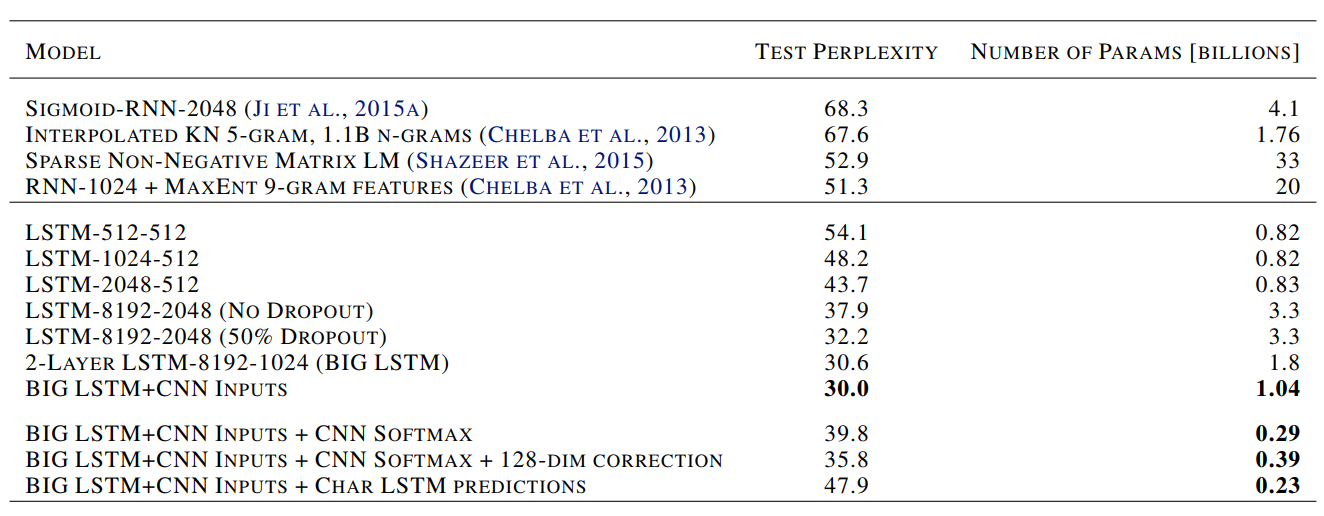
\includegraphics[width=12cm, height=5cm]{ComputationalLinguistics/Pictures/lm-stat.png}
\end{frame}

\appendix
\section<presentation>*{\appendixname}
\subsection<presentation>*{Useful links}

\begin{frame}[allowframebreaks]
  \frametitle<presentation>{Полезные ссылки}
    
  \begin{thebibliography}{10}
{
  \beamertemplatebookbibitems
  % Start with overview books.
    
\bibitem{jurafsky}
  \texttt{Speech and Language Processing. Daniel Jurafsky, James H. Martin. Chapter 3}
  \newblock \href{https://web.stanford.edu/~jurafsky/slp3/3.pdf}{\texttt{https://web.stanford.edu/\~jurafsky/slp3/3.pdf}}

\bibitem{jurafsky}
  \texttt{Exploring the Limits of Language Modeling}
  \newblock \href{https://arxiv.org/pdf/1602.02410.pdf}{\texttt{https://arxiv.org/pdf/1602.02410.pdf}}
}

    
  \end{thebibliography}
\end{frame}

\end{document}


